\documentclass[a4paper]{article}

%% Language and font encodings
\usepackage[english]{babel}
\usepackage[utf8x]{inputenc}
\usepackage[T1]{fontenc}
\usepackage{hyperref}

%% Sets page size and margins
\usepackage[a4paper,top=3cm,bottom=2cm,left=3cm,right=3cm,marginparwidth=1.75cm]{geometry}

%% Useful packages
\usepackage{amsmath}
\usepackage{graphicx}
\usepackage{url}
\usepackage{listings}
\usepackage{enumitem}

%% Solidity highlighting for listings
% Copyright 2017 Sergei Tikhomirov, MIT License
% https://github.com/s-tikhomirov/solidity-latex-highlighting/

\usepackage{listings, xcolor}

\definecolor{verylightgray}{rgb}{.97,.97,.97}

\lstdefinelanguage{Solidity}{
	keywords=[1]{anonymous, assembly, assert, balance, break, call, callcode, case, catch, class, constant, continue, contract, debugger, default, delegatecall, delete, do, else, event, export, external, false, finally, for, function, gas, if, implements, import, in, indexed, instanceof, interface, internal, is, length, library, log0, log1, log2, log3, log4, memory, modifier, new, payable, pragma, private, protected, public, pure, push, require, return, returns, revert, selfdestruct, send, storage, struct, suicide, super, switch, then, this, throw, transfer, true, try, typeof, using, value, view, while, with, addmod, ecrecover, keccak256, mulmod, ripemd160, sha256, sha3}, % generic keywords including crypto operations
	keywordstyle=[1]\color{blue}\bfseries,
	keywords=[2]{address, bool, byte, bytes, bytes1, bytes2, bytes3, bytes4, bytes5, bytes6, bytes7, bytes8, bytes9, bytes10, bytes11, bytes12, bytes13, bytes14, bytes15, bytes16, bytes17, bytes18, bytes19, bytes20, bytes21, bytes22, bytes23, bytes24, bytes25, bytes26, bytes27, bytes28, bytes29, bytes30, bytes31, bytes32, enum, int, int8, int16, int24, int32, int40, int48, int56, int64, int72, int80, int88, int96, int104, int112, int120, int128, int136, int144, int152, int160, int168, int176, int184, int192, int200, int208, int216, int224, int232, int240, int248, int256, mapping, string, uint, uint8, uint16, uint24, uint32, uint40, uint48, uint56, uint64, uint72, uint80, uint88, uint96, uint104, uint112, uint120, uint128, uint136, uint144, uint152, uint160, uint168, uint176, uint184, uint192, uint200, uint208, uint216, uint224, uint232, uint240, uint248, uint256, var, void, ether, finney, szabo, wei, days, hours, minutes, seconds, weeks, years},	% types; money and time units
	keywordstyle=[2]\color{teal}\bfseries,
	keywords=[3]{block, blockhash, coinbase, difficulty, gaslimit, number, timestamp, msg, data, gas, sender, sig, value, now, tx, gasprice, origin},	% environment variables
	keywordstyle=[3]\color{violet}\bfseries,
	identifierstyle=\color{black},
	sensitive=false,
	comment=[l]{//},
	morecomment=[s]{/*}{*/},
	commentstyle=\color{gray}\ttfamily,
	stringstyle=\color{red}\ttfamily,
	morestring=[b]',
	morestring=[b]"
}

\lstset{
	language=Solidity,
	backgroundcolor=\color{verylightgray},
	extendedchars=true,
	basicstyle=\footnotesize\ttfamily,
	showstringspaces=false,
	showspaces=false,
	numbers=left,
	numberstyle=\footnotesize,
	numbersep=9pt,
	tabsize=2,
	breaklines=true,
	showtabs=false,
	captionpos=b
}
\lstset{escapeinside={<@}{@>}}

\title{\vspace{3.0cm}\textbf{Solitor: Runtime Verification of Smart Contracts}\\
\large On the Ethereum network \\}

\author{Lars Stegeman\\ l.stegeman@student.utwente.nl}
\date{\vspace{0.5cm}\today}

\begin{document}
\begin{titlepage}
\maketitle
\vspace{1.5cm}
\begin{center}
\textbf{Master Thesis}\\
Master of Computer Science\\
Methods and tools for verification specialization\\
\vspace{0.5cm}
\textbf{University of Twente}\\
Faculty of Electrical Engineering, Mathematics and Computer Science\\
Formal Methods and Tools research group\\
\end{center}
\vfill
\textbf{Supervisors}\\
prof.dr. J.C. van de Pol, University of Twente\\
dr. M.H. Everts, University of Twente\\
\end{titlepage}

\newpage
\section{Abstract}
In this paper the tool Solitor is presented. Solitor is short for Solidity (runtime) monitor. It is a tool developed specifically for smart contracts on the Ethereum network. Solitor can parse and translate annotations in Solidity contracts to generated Solidity code which checks the expressions at runtime. Annotations can be used to check if certain properties hold during execution of the smart contract. These can either be contract invariants or pre and postconditions for methods. To recognize the annotations the original Solidity grammar is extended and is similar to that of the Java Modelling Language (JML). \par
The rest of this paper explains the background of the Ethereum network and how smart contract execute on the blockchain. This is important because smart contracts are committed to the blockchain. This means they are public and unchangeable. Ensuring the contract executed like intended is important because vulnerabilities can not be easily solved. Furthermore the report describes two case studies, where the tool is used to specify correct behaviour or detect a vulnerability. 
\newpage
\tableofcontents
\newpage

\section{Introduction}
Ethereum is a well known blockchain based cryptocurrency. In contrast to Bitcoin it is more focussed to be a smart contract platform. On this platform applications will run without any trusted central party. This makes these applications unstoppable and censorship resistant. Each day new smart contracts are deployed to the Ethereum network. Some of these smart contracts control a large sum of ether. Since this ether has real world value and the source code for smart contracts is in the open many people are finding vulnerabilities within contracts. Several high profile security bugs were found and exploited \cite{parity1, parity2,hkg,dao}. This sparked the interest in static analysis tools and formal verification of smart contracts. Many different analysis tools have already been developed. Static analysis tools can be executed on many contracts and detect mistakes by analysing known vulnerable patterns. Other tools which use formal verification need a specification to be able to guarantee a contract behaves the correct way. These specifications are usually written in another language or defined at the EVM level. This makes it hard to understand what properties are proven and what that means for the contract. More examples of tools can be found in Section \ref{sec:RelatedWork}. 

\subsection{Goal}
The goal of this research is to develop a tool that can do runtime verification for smart contracts. The annotations to check properties can be written at the level of Solidity. This will make it easy for Solidity developers to use the tool. Furthermore the specification does not have to be complete and proven correctly against all specifications like in the case of formal verification tools. This makes it easy to check for certain properties without having to specify all the behaviour. The generated code will be Solidity which can be executed on the blockchain like any normal contract. The tool will be made specifically for the language Solidity and for the Ethereum blockchain.
The benefits of this approach are:
\begin{itemize}
  \item Explicitly writing a specification helps understanding the problem. The code usually describes how a contract should behave and do calculations. While the specification should describe what the contract does and what properties should be satisfied.
  \item Runtime exceptional state. While the contract is active on the main Ethereum network properties can be checked at runtime. If a certain property fails due to an untested case, the program can go into an exceptional state. In this state, functions can be deactivated or the contract can be completely cleared. Some special form of governance can be coded in this state which requires human intervention before the contract will continue.
  \item The annotations can be used by static analysis tools for other purposes.
\end{itemize}

\subsection{Research Questions}
A runtime verification tool for smart contracts has to be usuable in the environment it will be used. The properties it can specify must be implementable in Solidity. This settings is much different from a normal general purpose programming language. For example the seperation of storage and memory is different. Contracts have to be annotated with a certain syntax. This syntax has to be designed in such a way that it is understandable and usable. Furthermore the usability of the tool as a whole should be tested on a case study of a smart contract.
More concrete the following questions are answered in this report:
\begin{enumerate}
\item \textbf{Property specification/definition.}
The first step is to decide and analyse which properties should be able to be checked and specified. Properties should make sense and should be able to be checked within Solidity. This raises the question:
\textit{What properties should the tool be able to identify and specify?}. Specifically the \textit{syntax} has to be defined. And a \textit{parser} has to be written to decide if properties are according to the defined syntax. 
\item \textbf{Tool development.}
The next step is defining the output of the tool. In other words: \textit{What can be generated from the specification and smart contract source code?}
\item \textbf{Tool usage on smart contract.}
The last step is to test the tool on real world smart contract. And see if it can detect vulnerabilities that would otherwise have not been found. \textit{How can the tool be used to detect vulnerabilities in smart contracts?}.
\end{enumerate}

\subsection{Report Structure}
This report will answer the above questions and introduce the tool Solitor. Before that some background information is given in Section \ref{sec:background}. This introduces the setting in which these smart contracts are executed. It explains the workings of the blockchain in combination of the executed code. The network state and contract state is explained in detail. Next the language Solidity is introduced in section \ref{sec:solidity}. This is the programming language that is most used to develop smart contracts on the Ethereum network. It compiles to the EVM (Ethereum Virtual machine) bytecode and is specifically designed for developing contracts. The language is introduced so that the design decisions for the tool can be understood. Section \ref{sec:tooloverview} discusses the tool in a high level overview. The next sections \ref{sec:annotationlanguage}-\ref{sec:generation} discuss the different phases in the tool process. Some of the limitations within Solitor are discussed in Section \ref{sec:limitations}. The tool is tested on two case studies. The first case study is a contract which models a subcurrency. This is called a token and many applications use such contract. The contract SimpleToken is a simplified version and a property is implemented and checked at runtime. The second case study is a contract which contains a vulnerability. The vulnerability is exposed using annotations. When executing the contract with annotations the vulnerability becomes visible and execution of the transaction is stopped. This can be seen in detail in Section \ref{sec:casestudy}. As said in the introduction many tools try to make smart contract development more secure. There are many approaches each focussing on a specific aspect of secure smart contracts. The different approaches and vulnerabilities they detect are discussed in Section \ref{sec:RelatedWork}. Lastly the conclusion of the report can be seen in Section \ref{sec:conclusion}. It briefly answers the questions asked in this introduction and discusses the results of Solitor. 

\newpage
\section{Background}
\label{sec:background}
This section will discuss the background information that will be built upon further in the document. First we will briefly discuss the important parts of the Ethereum Blockchain. Then we will discuss the smart contracts in more detail.
\subsection{The Ethereum blockchain}
The Ethereum platform is built upon a distributed public ledger. On this ledger the cryptocurrency ether is stored. Ethereum has different denominations of the unit ether. The smallest value or base value is called \texttt{wei}, a single ether represents 1e18 wei. In contrast to Bitcoin, it is an account based system and not based on unspent transaction outputs (UTXO). There are two types of accounts, one is a default account in which a user controls the spending of funds through its private keys. These accounts are called "Externally owned Accounts". An account can be referenced by its address which is a hashed version of the public key. Each address has a balance and a nonce. The nonce is incremented each time the balance is updated with a transaction. The other option is a "Contract Account", which means that it is managed by code only. A contract account has more data stored on the blockchain. These include storage hash and a code field. The code is set when the contract is constructed and initialized on the blockchain, and after that can never be changed. The code that is included in contracts is called Ethereum Byte Code. This bytecode is executed in a VM called the Ethereum Virtual Machine (EVM). Each contract has a persistent storage which is also maintained on the blockchain. Contract accounts only execute code when they are called from other contracts.\par
Transactions are created and sent to the network by creating a message and signing it with the private key of an "Externally Owned Contract". This contains information like the amount of ether and the receiver of the transaction. Additionally it can contain so called call data. This data is interpreted by the contract code and the correct function is executed. Transactions are the only entity that make changes to the storage. At an higher level overview we could see the Ethereum network as a large state machine in which changes to the state are controlled by transactions. Transactions are grouped in blocks and these blocks are distributed over the network and validated by each node. \par
The different types of state and environments are also described more formally in the Ethereum Yellow Paper \cite{wood2014ethereum}. The Yellow Paper states that there are three separate storages in each context.
\begin{itemize}
    \item World state ($\sigma$): A mapping of Ethereum addresses to the accounts. Within each account the balance, contract storage, contract code and nonce are stored. For "Externally Owned Account" the contract code and storage are empty.
    \item  Machine state ($\mu$): State of the currently executing code from a transaction. This includes program counter, contract memory and virtual machine.
    \item Execution Environment (I): Variables related to this transaction. For example caller address, amount of ether send and call data.
\end{itemize}
Transactions can only be initiated from accounts. This means that the blockchain is global state computer which changes each time a transaction is executed. Transactions can be seen as function calls with additional information. This information includes the transaction sender, gas price and amount of ether.\par
Blocks serve the purpose to group transactions and give them order. Because the ordering is very important to the outcome of the transactions. The ordering is determined within a block and should be deterministic and all nodes should agree on the global state. This securing of blocks is done using a proof of work mechanism that is used by most cryptocurrencies. However each miner also has to validate each transaction by executing the corresponding EVM code and adjusting the global state. This is also done by each individual node to validate the block which includes all the transactions.

\subsection{Smart Contracts}
Smart contracts are usually mentioned together with Ethereum. Other terms for smart contracts are "autonomous agents" or "executable code on the blockchain". It has many application domains according to the Ethereum White Paper \cite{buterin2013ethereum}. Examples of usage cases include token systems, decentralized autonomous organizations (DAO), financial derivatives, identity/reputation systems and decentralized file storage. The idea is that these domains are perfect for the blockchain since they take away the untrusted third party. Smart contracts can only operate on data within the blockchain, this means that all information has to be included in the transactions that are send from "externally owned accounts". However in this paper we will look at the functional capabilities of smart contracts on the Ethereum network. \par 
Smart Contracts on the Ethereum network consist of two parts. Each contract has a set of functions and a storage. The contract set of functions is defined by the contract code that is deployed with the contract creation. This contract code is EVM bytecode and is usually compiled from a higher level programming language. When the contract is created the storage is initially empty. Only the contract code can make changes and add data to the persistent storage, within this storage the state of the contract is maintained. As explained before each transaction also has a state. This is called \texttt{memory}, and is initially empty. It can also be used to store data and is much cheaper in terms of gas cost. But this data is not persistent through transactions, it is only persistent within the transaction. There are also so called "logs", this storage can only be used to store data and not retrieve. This storage is usually used to provide data for the external world because it can be searched efficiently.\par
Since the EVM is a turing complete language any program can be expressed within the platform. To mitigate the possibility of a Denial-of-Service attack (with for example an infinite loop) the principle of gas is introduced in Ethereum. Gas is used to limit the amount of complex code that can be executed within a single transaction. Each transaction only has a specified limit called the gas limit. If an execution is terminated unexpectedly or runs out of gas the complete transaction is reverted. This includes storage changes made before the exception. When a transaction is successful left over gas will be returned to the sender. In the case of an exception all the remaining gas is consumed.
Functions are only executed when they are called by external contracts. For example if a fund is to be released after a certain amount of time (block number higher then a certain amount). These funds will not be automatically transferred once the time threshold is reached, they will only be released when the function is called again.\par

\subsection{Smart Contract bugs}
Many smart contracts are deployed to the Ethereum main network every day. When a contract is created on the blockchain the contract code is stored on the blockchain forever. This cannot be changed afterwards. Because of this limitation bugs within smart contracts can be very costly. In the past many vulnerabilities have been detected causing a loss of several million Ether. This paper will not enumerate all of them since many other articles do a good job of summarizing all the found vulnerabilities. For a complete overview see \cite{dika2017ethereum} section 3, where each attack with its corresponding vulnerability is explained in detail.

\newpage
\section{Solidity}
\label{sec:solidity}
The most used language to develop contracts on Ethereum is Solidity \cite{solidityreadthedocs}. Solidity comes with a compiler that compiles Solidity code into EVM bytecode. This bytecode is what is executed and put on the blockchain. Solidity has features like control flow, types and different storage constructions. Additionally it has some global variables that apply only to the blockchain setting. In this section we will further introduce the language in detail.
\subsection{Syntax}
The syntax that is used by Solidity is heavily inspired by Javascript. Solidity is in contrast to Javascript strongly typed. It offers the common types in normal programming languages like; booleans, integers, strings, fixed point numbers. Since each contract is executed on the blockchain, storage is extremely costly in terms of gas cost. This is why many different sizes for integers exist: \texttt{uint8}, \texttt{int8}, \texttt{uint16}, until \texttt{uint256} and \texttt{int256}. \par
Solidity offers a number of different options for more complex types. These complex types have an extra annotation that defines their storage location. This can either be \texttt{storage} or \texttt{memory}. 
\begin{itemize}
    \item Structs are a form to create new types in Solidity. Structs can contain any type including mappings except itself. For example a struct type A cannot contain a member of type A (no recursive definition).  
    \item Arrays can be defined in memory or storage. Storage arrays can hold arbitrary types, memory arrays can not contain mappings. Storage arrays can be dynamically increased in size, however memory arrays are always fixed length.  
    \item Mappings can only be defined in storage. They map a key of a certain type to a value of another type. They can be compared to hash tables in normal programming languages. However the key set of a mapping is not stored, this makes mappings not iterable. 
\end{itemize}
The code snippet below shows how all these constructions can be used within a contract.
\begin{lstlisting}[
    language=Solidity
]
pragma solidity ^0.4.23;

contract C {
  // State variables are always stored in storage
  uint256 public number;
  uint[] x; 
  mapping(address => uint256) myMap;
  // Definition of type myStruct
  struct myStruct{
    uint256 a;
    address b;
  }

  // the data location of memoryArray is memory
  function f(uint[] memoryArray) public {
    x = memoryArray; // works, copies the whole array to storage
    var y = x; // works, assigns a pointer, data location of y is storage
    y[7]; // fine, returns the 8th element
    y.length = 2; // fine, modifies x through y
    delete x; // fine, clears the array, also modifies y
    // The following does not work; it would need to create a new temporary /
    // unnamed array in storage, but storage is "statically" allocated:
    // y = memoryArray;
    // This does not work either, since it would "reset" the pointer, but there
    // is no sensible location it could point to.
    // delete y;
    g(x); // calls g, handing over a reference to x
    h(x); // calls h and creates an independent, temporary copy in memory
    
    // Declaring a mapping in memory is not allowed
    // mapping(address => uint256) memory temp_map;
    
    myStruct memory a; // declares a variable of type struct in memory
    myStruct b; // default of complex types is storage
    b.a = 100; // will assign 100 to the variable number!
  }

  function g(uint[] storage storageArray) internal {}
  function h(uint[] memoryArray) public {}
}
\end{lstlisting}

\subsection{Structure}
In Solidity contracts are treated like objects in Object Oriented Programming languages. Contracts can contain state variables and functions and inheritance is supported between multiple contracts. A contract can have a constructor which will be called upon creation of the contract on the blockchain. In the code example below a simple contract is shown with the basic structure.
\begin{lstlisting}[
    language=Solidity
]
pragma solidity ^0.4.23;

contract SimpleStorage {
  uint public storedData; // State variable
  
  //Constructor will be called upon creation on blockchain.
  constructor(uint data){ 
    storedData = data;
  }
  
  function setData(uint data) public{
    storedData = data;
  }
  function() payable{
    //Unnamed function will be called if no function signature matches
  }
}
\end{lstlisting}
Solidity also has different visibility keywords. Their behaviour is a bit different from normal programming languages since it is executed on a blockchain setting. Visibility can be defined for functions and variables.
\begin{itemize}
    \item \texttt{external}: External can only be used by functions and means that they can not be called from internal functions. They can be called from other contracts.
    \item \texttt{public}: Public can be used for functions and state variables. For functions it means that it can be called both internal and external. For state variables it means that a getter function is automatically generated.
    \item \texttt{internal}: Internal functions and state variables can only be accessed internally from within the current contract and derived contracts.
    \item \texttt{private}: Private functions and state variables are only visible to the contract they are defined in.
\end{itemize}
The extra keywords are used because different functionality can be desired by contracts. Also note that private variables can be read outside of the EVM by inspecting the storage of the smart contract \footnote{For example with the web3.js interface with the call \texttt{web3.eth.getStorageAt(addressHexString, position)}}\par
Solidity also gives the possibility to define function modifiers. These are usually used to check a condition before execution of a function. Modifiers can be inherited from other contracts and reused in functions on that contract. As explained in the previous section the Ethereum blockchain has another type of storage called "logs".  Logs are read only and can be written to using \texttt{Events}. Events have to be defined in the contract itself and can be inherited, events can have specified parameters to emit the correct information. Below is a Solidity code snippet showing the basic behaviour of both constructions.
\begin{lstlisting}[
    language=Solidity
]
pragma solidity ^0.4.23;

contract myContract {
  uint public data; 
  
  //Event declaration
  event dataIncreased(address sender, uint amount);
  
  //Modifier declaration
  modifier onlyPositive(uint number){
    require(number >  0);
    _;
  }
  
  //Before function call check modifier onlyPositive
  function increment(uint number) onlyPositive(number) public{
    data +=number;
    //Emit event dataIncreased
    emit dataIncreased(msg.sender,number);
  }
} 
\end{lstlisting}
The function \texttt{increment} has a modifier that will be executed when the function is called. The modifier \texttt{onlyPositive} checks the number and requires the number to be greater then zero. The "\_;" indicates the rest of the body of the function. This way function modifiers can be used to add code before and after the normal function body. If the assumption fails the require will throw an exception and the transaction will stop executing. This means that all state changes made during the transactions are reverted and the transaction is marked as failed. There are two types of constructions that can be used to detect undesired behaviour one is \texttt{require()} the other is \texttt{assert()}. Both function will throw an exception when the statement is false, but assert will consume all remaining gas while require will not consume any more gas. This means that in practice \texttt{require} is used to check and validate user input, and \texttt{assert} is used to test invariants and internal error checking. Both functions will create an exception that will bubble up to through the call structure. At this point exceptions can not be caught.

\subsection{Blockchain specific variables}
What makes Solidity special in terms of programming languages is that it is executed on the blockchain. All code is executed because of the transactions that are being sent to the network. These transactions can be seen as rich function calls with extra information. This extra information is available in special constructed variables which are globally accessible during execution of the contract.\par
There are two objects that contain information about the blockchain these are: \texttt{block} and \texttt{msg}. The block object contains variables like \texttt{block.number}, \texttt{block.timestamp}, \texttt{block.difficulty} and \texttt{block.coinbase} (current block miner address). The information in block is the block where the current transaction is mined in. The object msg contains information about the current transaction. These are found in variables like: \texttt{msg.gas} (remaining gas), \texttt{msg.value} (value sent in wei) and \texttt{msg.sender} (address of the sender).
The \texttt{address} object is used for communication between contracts. This makes it possible to execute code of multiple contracts within a single transaction. The keyword \texttt{this} refers to the address object of the current contract. This also contains the balance of the contract under the variable \texttt{<address>.balance}. There are five different flavors of calling other contracts.
\begin{itemize}
    \item \texttt{<address>.transfer(uint256 amount)}: forwards given amount in wei to address, throws on failure. The function sends 2300 gas with the transfer. 
    \item \texttt{<address>.send(uint256 amount) returns (bool)}: same behaviour as transfer but returns false on failure.
    \item \texttt{<address>.call(...) returns (bool)}: forwards all gas to function call. Returns false on failure.
    \item \texttt{<address>.delegatecall(...) returns (bool)}: same behaviour as call but storage and state variables of original contract are used. This makes it possible to create library functionality within the blockchain. The library contract can contain functions that do not require access to state variables. That means that they must rely on their input. Or the library contract has to have to exactly the same state variables declared in order to be used in functions of the library contract.
    \item \texttt{<address>.callcode(...) returns (bool)}: older version of delegatecall. Usage is discouraged and will be removed in the future.
\end{itemize}
All these transfer functions can be sent to "Externally Owned Contracts", but also on "Contract Accounts". This means that arbitrary code can be executed when invoking one of these methods. To limit the amount of code that can be executed by a remote function call it is important to specify the amount of gas to be sent with the transfer. Exceptions can not be caught within contracts, they bubble up through the call tree. Exceptions can be caught when using the \texttt{send} function because then this will return false instead of rethrowing/passing on the exception which is what the \texttt{transfer} method does.

\newpage
\section{Tool Overview}
\label{sec:tooloverview}
% \begin{itemize}
%   \item Tool works in two phases validation and generation.
%   \item Validation typechecks and checks if annotations are well formed according to grammar.
%   \item Generation generates original solidity code with extra added code to check annotations at runtime.
%   \item Approach uses a Solidity grammar that can be updated easily for future updates.
%   \item Output of validation phase can be used for other verification tools (result is a parse tree).
%   \item Annotations can be defined as invariants and pre or post conditions for functions.
%   \item Annotations use JML like syntax.
%   \item Tool can be used both during development (as extra test cases) or on the actual live blockchain (this probably costs a lot of extra gas = ether).
% \end{itemize}
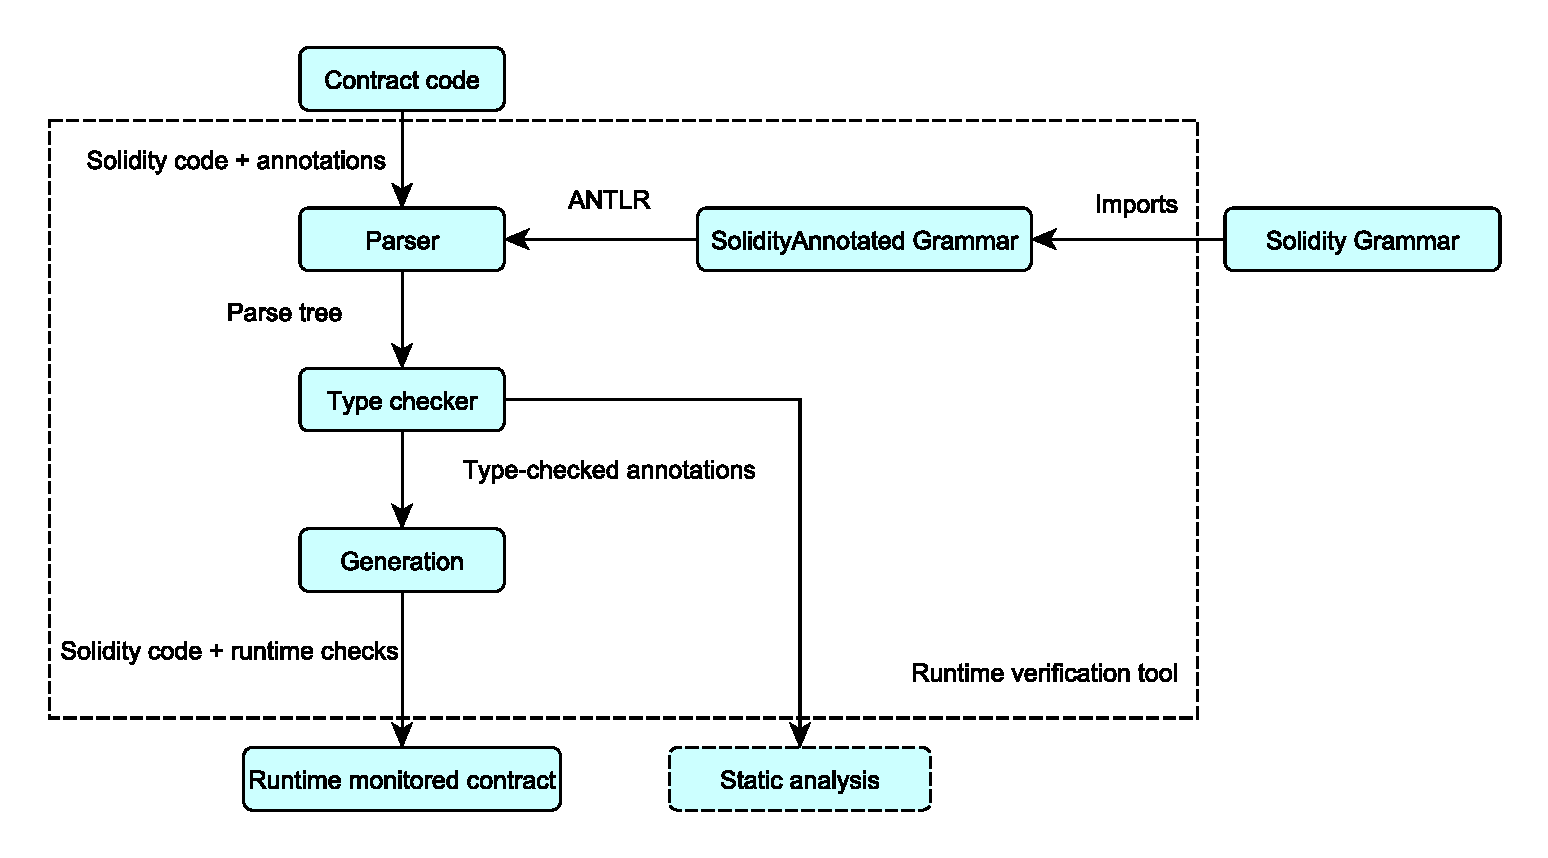
\includegraphics[width=\textwidth,height=\textheight,keepaspectratio]{resources/ToolOverview.eps} 
In the picture the complete overview of the tool can be seen. Within the dashed square the implemented parts are visible. The arrows indicate the flow of the contract code throughout the program. \par
First contract code has to be annotated according to a specified grammar. Section \ref{sec:annotationlanguage} explains the grammar in more detail and gives some example annotations. The tool ANTLR \cite{parr2013definitive} is used to generate code for the lexer and parser. The grammar has to be expressed in the language that is recognized by the ANTLR tool. The automatically generated parser is used to parse Solidity contract code and annotations into a parse tree. The parse tree makes it able to walk the complete contract code and do analysis on specific parts of the contract. This parse tree is used in later stages of the tool. \par
The next step is type checking the annotations. This uses the parse tree to examine the annotations and check if they are valid. The type checking is done bottom up and works in two phases. The first phase collects all the relevant variables. This includes state variables and function definitions (function name, arguments and return values). The next phase uses this information to do the actual type checking of the annotations. This is explained in more detail in Section \ref{sec:typechecker}. \par
The result of the type checker phase are type-checked annotations. In practice these are parse tree objects in which the types correspond to the operators used and the identifiers that are used are also defined in the contract. This is used as input for the generation phase. The generation phase will operate on the information that is created during the type checker phase. For each annotation it will generate the code that is needed to check it during runtime. This happens in a single pass of the complete parse tree. Details on this phase can be found in Section \ref{sec:generation}. \par
The output of the type checker phase can also be used for static analysis tools. The benefit of using the tool to validate the annotations is that the result is a type checked parse tree that can be parsed and traversed in various ways to be useful for static verification methods. 

\newpage
\section{Annotation Language}
\label{sec:annotationlanguage}
The first step towards implementing the tool is to define an annotation syntax, and formally write this down using a grammar. The parser generator that is used is called ANTLR \cite{parr2013definitive}. Using the grammar definition the lexer and parser will be automatically generated. The output of this phase is a parse tree that can be used in later stages of the tool.

\subsection{Grammar definition}
There already exists a grammar for the complete Solidity language \cite{antlroriginalgrammar}. This grammar is expressed in the language that is used by ANTLR tool. ANTLR has the capabilities to extend certain grammars. This is done by inheritance over the original grammar. This principle is explained in detail here \footnote{\url{https://github.com/antlr/antlr4/blob/master/doc/grammars.md}}. It functions much like object oriented inheritance. The main grammar inherits all rules, token specifications and named actions from the imported grammar. Rules in the main grammar override rules in the imported grammar. We will use this principle to extend the grammar of Solidity to recognize the special annotations that will later be used in the tool. In this case the imported grammar is the original Solidity grammar. The 'new' main grammar is defined further below and is called SolidityAnnotated. The advantage of this approach is that changes to the original Solidity grammar can easily be updated in the tool. This only holds for small changes to the language, if grammar rules that the tool makes use of the SolidityAnnotated grammar also has to be updated.\par
The annotations have certain requirements that can be summarized the following way. Later each requirement is discussed in detail.
\begin{itemize}
    \item Annotations can be specified at the top level of the contract.
    \item Annotations should be able to reference all variables used in the contract.
    \item Basic math operations can be used within annotations.
    \item Annotations can not have side effects.
    \item The type should be boolean at the highest level (that way they can be verified).
    \item There are two types of annotations: invariants and pre- or postconditions to a function.
\end{itemize}

The annotation syntax is heavily inspired from the JML annotation syntax \cite{leavens2008jml}. But has a lot less built in keywords since the setting is easier and the tool is less complex. \par
The original Solidity grammar is extended in such a way that annotations can only be defined on the top level. The relevant parts of the original Solidity grammar can be seen in the snippet below. This does not include the full grammar specification but only the parts that are relevant for the annotation syntax.

\begin{lstlisting}[basicstyle=\ttfamily]
grammar Solidity;

sourceUnit
  : (pragmaDirective | importDirective | contractDefinition)* EOF ;

contractDefinition
  : ( 'contract' | 'interface' | 'library' ) identifier
    ( 'is' inheritanceSpecifier (',' inheritanceSpecifier )* )?
    '{' contractPart* '}' ;

contractPart
    : stateVariableDeclaration
    | usingForDeclaration
    | structDefinition
    | constructorDefinition
    | modifierDefinition
    | functionDefinition
    | eventDefinition
    | enumDefinition ;
\end{lstlisting}
In the original grammar the definition of \texttt{contractPart} is what defines the declaration of variables and the definitions for structs and functions. This is where the extra annotations have to be added to the grammar. The snippet below shows the basic definition of an annotation. This is not the complete grammar: some of the tokens are omitted from this snippet, since they are not required to understand the grammar definition.
\begin{lstlisting}[basicstyle=\ttfamily, breaklines=true]
grammar SolidityAnnotated;
import Solidity;

@header {package generated;}

//Added annotationDefinition. This enables annotations to be on the top level only.
contractPart
  : stateVariableDeclaration
  | usingForDeclaration
  | structDefinition
  | constructorDefinition
  | modifierDefinition
  | functionDefinition
  | eventDefinition
  | enumDefinition 
  <@\textcolor{red}{  | annotationDefinition ;}@>

annotationDefinition
  : AnnotationStart AnnotationKind annotationExpression;

// Same as the expression rule except it does not include assignments, only comparisons
annotationExpression
  : '(' annotationExpression ')'
  | '!'annotationExpression
  | ('\\forall' | '\\exists') '(' identifier 'in' identifier ':' annotationExpression')'
  | annotationExpression integerOpInteger annotationExpression
  | annotationExpression integerOpBoolean annotationExpression
  | annotationExpression compareOp annotationExpression
  | annotationExpression booleanOp annotationExpression
  | primaryAnnotationExpression;

primaryAnnotationExpression
  <@\textcolor{red}{: primaryExpression}@> 
  | primaryAnnotationExpression '.' <@\textcolor{red}{identifier}@> 
  | primaryAnnotationExpression '[' primaryAnnotationExpression ']'
  | '\\old' '(' primaryAnnotationExpression ')';

//Annotation Tokens
AnnotationStart
  : '//@';

AnnotationKind
  : 'inv'| 'pre'| 'post';

// Added '->' for then.
booleanOp
  : '&&' | '||' | '->';

compareOp
  : '==' | '!=';

integerOpBoolean
  : ('>'|'>='|'<'|'<=');

integerOpInteger
  : '+' | '-';

// Remove '@' from first position of LINE_COMMENT token. 
LINE_COMMENT 
  : '//' ~[@] ~[\r\n]* -> channel(HIDDEN);
// Send whitespace to channel hidden.
WS
  : [ \t\r\n\u000C]+ -> channel(HIDDEN);
\end{lstlisting}
An AnnotationDefinition is composed of multiple components. It has a \texttt{AnnotationStart}, \texttt{AnnotationKind} and \texttt{annotationExpression} component. The \texttt{AnnotationStart} token is used to signal that an annotation definition is coming next. This is defined as '//@' making it a line comment to other solidity compilers. This makes annotated solidity code still compilable by normal Solidity compilers. For the grammar to accept this notation the \texttt{LINE\_COMMENT} token has to be adjusted to not accept '@' as a second character. Otherwise all annotation comments would be recognized as a \texttt{LINE\_COMMENT} making it unusable. \par
There are three types of annotations that are defined by the token \texttt{AnnotationKind}. They can either be an invariant or a pre- or post-condition of a function. Invariants are defined per contract, and should hold at any point during the execution of the contract. Pre- or post-conditions are defined for a specific method. They are checked before and after execution of the method. Each annotation has an expression which has to be evaluated called \texttt{annotationExpression}. The expression parser rules are separated between \texttt{annotationExpression} and \texttt{primaryAnnotationExpression}. This is needed to keep the hierarchy in parsing and prevent using complex expressions within primary definitions. For example using the keyword '\textbackslash old' before parenthesis. The annotation expressions use a different parser rules than the expression rules that are used within the original Solidity grammar. The \texttt{annotationExpression} does not allow syntax like \texttt{expression + '++'} and to distinguish these a new parser rule was introduced for annotations only. \par
The order in which the different subrules are defined in the \texttt{annotationExpression} is imported. The order indicates the priority which the subrules are given. This means that parenthesis bind stronger then any other rule, this is followed by \texttt{!} and so on. The \texttt{annotationExpression} construction contains all the logical comparators that can be used within annotations. In general they are of the form \texttt{expression - <operand> - expression}. The expression are defined recursively thus making it able to form longer expressions with multiple operands. The parser rules in \texttt{primaryAnnotationExpression} are used as leaves in the expression. \texttt{primaryExpression} reverts to different kinds of literals that are used in Solidity. The other rules deal with complex types of Solidity and the possibility to reference an old variable.  
\texttt{primaryExpression} and \texttt{identifier} are parser rules that are defined in the original Solidity grammar. The annotation expressions make use of these rules so that they do not have to be defined again. These rules do not include assignments and are without side effects. The \texttt{primaryExpression} parser rule includes all the literals that can be used within Solidity. The parser rule \texttt{identifier} is used for all kinds of identifiers such as function identifiers and variable identifiers. Function calls are not allowed within annotations, for more details see Section \ref{sec:limitations}.

\subsection{Examples}
In this section a couple of annotation examples will be given for example contracts. First a contract snippet is shown and later the meaning of this annotation is explained.
\lstinputlisting[language=Solidity, linerange={4-6}]{examples/BasicAnnotations.sol}
Defines an invariant that will be checked at the start and end of every function. \texttt{nr1} and \texttt{nr2} are global contract variables. \texttt{nr1} should always be bigger than \texttt{nr2}.
\lstinputlisting[language=Solidity, linerange={9-13}]{examples/BasicAnnotations.sol}
Defines a post condition on the function \texttt{doSomething()}. Checks if the owner is not changed during execution of the function.
\lstinputlisting[language=Solidity, linerange={14-16}]{examples/BasicAnnotations.sol}
Defines an invariant that will check if all elements in array \texttt{a} are positive.
\lstinputlisting[language=Solidity, linerange={19-23}]{examples/BasicAnnotations.sol}
Postcondition for the function \texttt{changeSomething()}. If the sender of this transaction is equal to the owner (\texttt{msg.sender}), variable \texttt{b} must be different from the start of the function. 
\lstinputlisting[language=Solidity, linerange={25-27}]{examples/BasicAnnotations.sol}
Example of a mapping that maps \texttt{address} to \texttt{uint256}. The invariant checks the key \texttt{adr} in the map and checks if it is equal to 5. \hfill\\
A few example of expressions that do not parse correctly:
\lstinputlisting[language=Solidity, linerange={4-9}]{examples/ParseError.sol}
Functions are not recognized in annotations. This is because some functions could have side effects. This can be checked in typechecker but is not implemented yet.
\lstinputlisting[language=Solidity, linerange={11-14}]{examples/ParseError.sol}
The construction \texttt{\textbackslash old()} can only reference primary expression and not complex expressions.

\newpage
\section{Type Checker}
\label{sec:typechecker}
\subsection{Design}
Annotations have to be validated on certain aspects for them to be meaningful. These aspects have to be verified first for the annotations to be useful in the next generation phase. The parser ensures annotations are syntactically correct however there are more properties that have to be checked. The typecheck phase will consist of two passes that walk the complete parse tree. The first walk will collect all the variables and defined structures and store these in an information object. The second walk will type check each annotation individually. During this type checking the type of each identifier is looked up using the collected information from the first walk. 
\subsection{Implementation}
During the first phase all the variables, structs and function definitions are stored in an object. This object is later used by the second phase to retrieve information.
\begin{lstlisting}[breaklines=true, language=Java ]
public class ValidationInformation {
  ArrayList<SolidityVariable> identifiers;
  ArrayList<SolidityFunction> functions;
  ArrayList<SolidityStruct> structs;

  ...
}
\end{lstlisting}
\begin{itemize}
  \item SolidityVariable is an object which has a name (the identifier) and a type. These model state variables in a contract.
  \item SolidityFunction is an object which represent a function and stores the name and arguments. The arguments are of type SolidityVariable.
  \item SoldityStruct is an object that represent struct definitions in a solidity contract. It stores the name and elements. Elements are again of type SolidityVariable.
\end{itemize}
Solidity has many types and to make generation and typechecking easier the types are reduced to 8 base types (\texttt{uint256, uint128} etc are all regarded as \texttt{INTEGER}). These are all represented in the enumeration \texttt{SolidityType}, and all the internal representation of contract code make use of it. The internal representations must deal with nested constructions. For example consider the following solidity code:
\begin{lstlisting}[breaklines=true, language=Solidity ]
struct A{
    B b;
}
struct B {
    uint256 nr;
}
A var1;
\end{lstlisting}
For this Solidity code the typechecker would create two \texttt{SolidityStruct} objects, \texttt{A} and \texttt{B}. Struct \texttt{B} contains a variable texttt{nr} of type \texttt{INTEGER}, struct \texttt{A} contains a variable \texttt{b} of type \texttt{STRUCT} with reference to \texttt{B}. There also is a global variable \texttt{var1} with type \texttt{STRUCT} with reference to \texttt{A}. \par
The next phase will only parse the annotation part of the contract code, this means that no original solidity contract code will be reached. This is where the actual typechecking happens. It works bottom up, getting the type of each identifier and verifies the types of each step. The top level of each annotation should result in the type \texttt{BOOLEAN}. An extra type \texttt{UNDEFINED} was added to the SolidityType object to deal with cases where the identifier was not found and to produce a result without crashing the program. For the rest of the parse rules/operators the following type system is used:
\begin{itemize}
  \item Base case: expression is a \texttt{primaryAnnotationExpression}. This could mean a identifier where the type is found through the \texttt{SolidityVariable} or a literal of some type. The type can just be passed on to the higher level.
  \item '!' \texttt{expression}: Type checker verifies the nested expression and validates this results in \texttt{BOOLEAN}. Result of this step is always \texttt{BOOLEAN}.
  \item \textbackslash forall | exists( identifier  in identifier: expression): There are multiple things that have to be verified. First the second \texttt{identifier} should be of type \texttt{MAPPING} or \texttt{ARRAY}. Secondly the nested expression is typechecked, this is within a special scope since expressions can make use of the first identifier. This expression should result in \texttt{BOOLEAN}. This result is also returned for the higher level expression.
  \item \texttt{expression} ('+' | '-') \texttt{expression}:Both subexpressions should return \texttt{INTEGER}. Result of the current expression is \texttt{INTEGER} aswell.
  \item \texttt{expression} ('>'|'>='|'<'|'<=') \texttt{expression}: Both sub-expressions should return \texttt{INTEGER}. Result of the current expression is \texttt{BOOLEAN}.
  \item \texttt{expression} ('==' | '!=') \texttt{expression}: The types of the sub-expressions should match. The result of this is \texttt{BOOLEAN}.
  \item \texttt{expression} ('\&\&' | '||' | '->') \texttt{expression}: Both sub-expressions should return \texttt{BOOLEAN}. Result of this is \texttt{BOOLEAN} aswell.
\end{itemize}
If any of the types do not correspond to the expected value a validation error is reported and logged. \par
In case complex types are used such as structs the additional information is retrieved from the corresponding object that is referenced. For example consider a identifier \texttt{a.b}. This would mean that the type of \texttt{a} must be a struct and that in the definition of the struct the type of the identifier \texttt{b} must be retrieved. Additionally annotations can make use of function arguments and reference them. This is solved by looking up the \texttt{SolidityFunction} object that the annotation was declared above. This makes it possible to retrieve the types of function arguments and use them within the annotation.

\newpage
\section{Generation}
\label{sec:generation}
% \begin{itemize}
%     \item Explain generation of functions for annotations. Each annotation will be transformed to a function, the function takes in arguments that are also generated automatically.
%     \item Explain how functions are calling the code for checking annotations. Original Function will be transformed to a private function and renamed to 'functionName"+ \_body. New function calls this function with the extra annotations.
%     \item Implementation of generation is using a TokenStreamRewriter (with whitespace) and an abstract parse tree (only tokens that are in grammar). Tokens in both structures know the position, this way the original solidity code can be printed and extra code can be added through traversing the parse tree.
% \end{itemize}
\subsection{Design}
The next step in the tool process is the generation phase. In this phase new code will be generated and added to the original contract. Requirements are that the interface of the contract does not change. Therefore we will warp the original function in a new function which calls the original function. The functional behaviour of the contract should remain the same and the added code only performs extra checks. For each added annotation three steps have to be performed:
\begin{enumerate}
  \item Generate a function for each annotation that checks the expression. This function should have the correct number of arguments that are used within the annotation. Arguments are variables that are not reachable from the global scope and used in the expression. These are \texttt{old} variables and function variables. The only variables that are available within a function with no arguments are the global defined variables. These do not have to be given as an argument since then you have two variables defined with the same name. Other variables have to be given as an argument to the function. This includes function arguments, these are arguments that the original function has where this annotation is defined for. This is empty by construction for invariants since they do not reference a function. Additionally pre- and postconditions can use the \textbackslash old() on a variable. This means the value of the variable before the function execution, and this has also to be given as an argument to the annotation function.
  \item For each original function of the contract: Create a wrapper function with the old name which calls the original function body.
  \item Add all annotations that should be checked to the wrapper function. All variables that should be stored before the function call should be stored in memory before executing the function body. This means that all variables that are reference in an annotation with the keyword \textbackslash old() have to be stored in a variable with name 'variable + \_old'.
\end{enumerate}
To illustrate the steps consider this small example:
\begin{lstlisting}[breaklines=true, language=Solidity ]
//@ inv 'invariant_expression'

//@ post 'post_expression'
function testFunction() public{
    //...
}
\end{lstlisting}
At the end of the generation phase this will be the generated code:
\begin{lstlisting}[breaklines=true, language=Solidity ]
//@ inv 'invariant_expression'
function annotation0(){
  //check 'invariant_expression'
}

//@ post 'post_expression'
function annotation1('argument'){
  // check 'post_expression'
}

function testFunction() public{
  //stored variables in memory, i.e. copy all variables in 'argument'
  annotation0();
  testFunction_body();
  annotation1('argument');
  annotation0();
}

function testFunction_body() private{
    //...
}
\end{lstlisting}

\subsection{Implementation}
During the typechecking phase the object \texttt{AnnotationInformation} is created for each annotation it parses. This object contains the following information:
\begin{lstlisting}[breaklines=true, language=Java ]
public class AnnotationInformation{  
  ParserRuleContext node;
  private String name;
  private Map<SolidityVariable, Boolean> variables;
  private String type;
  private String function;

  ...
}
\end{lstlisting}
\begin{itemize}
  \item Reference to the node in the parser tree.
  \item A unique name for the annotation. This name is generated and is 'annotation' + a number.
  \item A list of arguments used in the method. The boolean indicates if it should be included as an argument for the method. As explained in the Design section. These are all arguments that cannot be reached from the global scope.
  \item Type of the annotation. Invariant, Pre or Post-condition. This indicates where it should be added to the wrapper function.
  \item Function the annotation is declared above. Null in case this is an invariant.
\end{itemize}
When parsing the tree the correct \texttt{AnnotationInformation} object is retrieved using the parse tree node. The function declaration is constructed using the name and arguments from this object. The body of this function can be constructed from the \texttt{expression} that is within the parse tree object. In most of the cases the code can directly be printed but in some cases the expression has to be altered:
\begin{itemize}
  \item The expressions \texttt{\textbackslash forall} and \texttt{\textbackslash exists} have to be replaced with a loop, that checks the expression for all the elements of the collection. 
  \item The usage of \texttt{\textbackslash old} has to be replaced with the variable that was created and initialized before the function execution. This means rewriting the variable \texttt{\textbackslash old(identifier)} to \texttt{identifier\_old}. In case of structs this is a bit more works since \texttt{\textbackslash old(a.b)} should be replaced with \texttt{a\_old.b}.
  \item Boolean operator \texttt{a->b} which can be used in annotations is not valid Solidiy code, and has to be replaced with \texttt{!a||b}
\end{itemize}
Since the annotations are type checked the generated code will always be valid. The result is always a boolean value. The actual testing of this value is done using an \texttt{assert} statement. If the value is false it means that the transaction will be reverted and all gas will be consumed. This could be changed to for example an \texttt{event}. The difference in approach is important. Assert will revert the entire transaction. A possible vulnerability that triggers the assertion will not go through as the assertion stops the execution. The vulnerability can not be exploited. In the case of changing this to an \texttt{event} the vulnerability can be exploited, but it will be registered because of the emitted event. Other behaviour can be specified here, for example calling a function that halts all the functionality of a contract except for a special function that only the admin of the contract can execute.\par
When the parser encounters a function it will check if annotations have to be added. This means searching through all \texttt{AnnotationInformation} objects and see if any of them reference the current function or are null (invariant). The original function will be transformed to a private function and renamed to 'functionName"+ \_body. The new wrapper function will call this function. The wrapper function does two other things that are important that is saving the current state of variables that are later to be used in annotations. It will only do this for variables that are referenced within \texttt{\textbackslash old(identifier)}. The second thing it does is add function calls to annotation before and after executing the original body. Annotations of type invariant are added before and after, preconditions only before and postconditions only after. \par
The actual printing of the contract code works with a \texttt{TokenStreamRewriter}\footnote{\url{https://www.antlr.org/api/Java/org/antlr/v4/runtime/TokenStreamRewriter.html}}, which is part of the ANTLR framework. The problem with printing the contract code is that the parse tree skips all whitespace. This means that the whitespace is lost in the parsing process. Including the whitespace in the parser rules would complicate the grammar because they have to be added to every rule. The ANTLR book also has an example on a similar case like this \footnote{Source code can be found here: \url{https://pragprog.com/titles/tpantlr2/source_code}. The example is in lexmagic/ShiftVarComments.java}. The idea is that the lexer gives all tokens a number in order, but the tokens are split between two channels. The parse tree only parses tokens on the first channel and ignores the others. The \texttt{TokenStreamRewriter} has the information of both channels. The token positions are still known and this way the \texttt{TokenStreamRewriter} can replace/insert text based on parser rule nodes positions. The tool uses the rewriter to insert the annotation blocks and function body in the correct places while preserving whitespace of the original contract code.

\subsection{Mappings}
\label{sec:mapping}
The above section holds for all constructions except for \texttt{mappings}. A mapping cannot be stored in memory and is not iterable since the key set is not known. This gives problems 1) when storing the variable for \texttt{\textbackslash old()} and 2) checking a expression for all elements in a mapping. \par
This is solved by using an iterable mapping \footnote{\url{https://github.com/szerintedmi/solidity-itMapsLib}}. This works by wrapping the mapping definition within a struct. This struct contains the mapping and an array. The array stores the indexes which are used. Since the indexes are in an array these can be iterated. The key and value can be retrieved using the index. The value can also be retrieved using the key. In order for this to work extra code has to be added to the contract.
\begin{itemize}
  \item Import the library at the beginning of the contract.
  \begin{lstlisting}[breaklines=true, language=Solidity ]
  import "./itMapsLib.sol";
  \end{lstlisting}
  \item Use library function when doing operations on the struct.
  \begin{lstlisting}[breaklines=true, language=Solidity ]
  using itMaps for itMaps.itMapUintUint;
  using itMaps for itMaps.itMapAddressUint;
  using itMaps for itMaps.itMapUintAddress;
  \end{lstlisting}
  \item Replace declaration of mapping with iterable mapping.
  \begin{lstlisting}[breaklines=true, language=Solidity ]
  //mapping(address => uint256) a;
  itMaps.itMapAddressUint a; 
  \end{lstlisting}
  \item Create mapping\_old for annotation purposes. Only when the mapping is used within a \textbackslash old() expression.
  \begin{lstlisting}[breaklines=true, language=Solidity ]
  itMaps.itMapAddressUint a_old; 
  \end{lstlisting}
  \item Replace each mapping reference with \texttt{.get(...)} or \texttt{.set(...)} depending on the context.
  \begin{lstlisting}[breaklines=true, language=Solidity ]
  //uint256 b = a[0x0];
  uint256 b = a.get(0x0);
  //a[0x1] = 1;
  a.set(0x1, 1); 
  \end{lstlisting}
\end{itemize}

\newpage
\section{Limitations}
\label{sec:limitations}
% mappings, contract inheritance, scoping, /result, timestamp
There are some limitations of Solitor that are present in the current version of the implementation. Some of the limitations are in the annotation language and some of them are because of the generated Solidity code. The annotation language and parser only work on a single scope level. This means each declared variable can only be used once. However in Solidity contract inheritance is supported. This makes it able to define small contracts and inherit from these contracts. This makes development of smart contracts modular and scalable. The tool currently does not support inheritance. This means that the tool only parses the main contract and does not look in the inheritance tree. Annotations can only make use of definitions that are declared within the current contract. To solve this problem the tool would have to be extended with a scope mechanism. Different variables are declared in different contracts and thus have a different scope. Annotations should be able to reference inherited properties and make use of the variables. This requires some changes to the parser structure, but not the annotation language. The parser should look up all the inheritance statements and parse all contracts that are referenced by \texttt{import} statements. These contracts can be declared in seperate files. \par
Since mappings are not iterable in Solidity these are replaced by iterable mappings as explained in Section \ref{sec:mapping}. However iterable mappings are only replaced for a few types of mappings. These are mappings which maps \texttt{uint $\Rightarrow$ address}, \texttt{address $\Rightarrow$ uint}, \texttt{uint $\Rightarrow$ uint}, all other combinations are not supported. Also nested mappings are excluded from the generation. The iterable mapping solution that is used in the current version of the tool uses a global variable to store the \textbackslash old state of the mapping. Using another function within a function which uses an  annotation would overwrite the global variable, making it unusable to check the annotation expression. This limitation is only due to the generation of Solidity code for the annotation. The annotation syntax can handle these nested mappings and other declared mappings. \par

\newpage
\section{Tool Usage}
The code of the tool is publicly available on the repository \url{https://github.com/LarsStegeman/EthereumRuntimeMonitoring}. Instructions on how to use the tool on other contracts can be seen in the README.

\hypertarget{getting-started}{%
\subsection{Getting Started}\label{getting-started}}

\hypertarget{prerequisites}{%
\subsubsection{Prerequisites}\label{prerequisites}}

\begin{itemize}
\item
  Java 1.8
\item
  Maven 3.5.3
\item
  ANTLR 4 (Maven will get this automatically when installing)
\end{itemize}

\hypertarget{installing}{%
\subsubsection{Installing}\label{installing}}

To install this tool perform the following steps

Clone this repository

\begin{verbatim}
git clone https://github.com/LarsStegeman/EthereumRuntimeMonitoring
\end{verbatim}

Build the tool using maven

\begin{verbatim}
mvn package
\end{verbatim}

Run the tool with basic example

\begin{verbatim}
mvn exec:java
\end{verbatim}

This should output the file \texttt{basicAnnotations\_generated.sol}.

\hypertarget{using-the-tool}{%
\subsection{Using the tool}\label{using-the-tool}}

\hypertarget{grammar-examples}{%
\subsubsection{Grammar examples}\label{grammar-examples}}

For example annotations see Section \ref{sec:annotationlanguage}. The grammar for the annotation
language can be found in the file
\href{https://github.com/LarsStegeman/EthereumRuntimeMonitoring/blob/master/src/main/antlr4/SolidityAnnotated.g4}{SolidityAnnotation.g4}. More
example annotations can be found in the \href{https://github.com/LarsStegeman/EthereumRuntimeMonitoring/tree/master/src/test/contracts}{test
directory}.

\hypertarget{run-the-tool-on-other-contracts}{%
\subsubsection{Run the tool on other
contracts}\label{run-the-tool-on-other-contracts}}

When the tool is build, a jar file is also generated to use the tool on
other contracts. The jar file is located in the \texttt{target}
directory. Use the tool on other contracts using the command

\begin{verbatim}
java -jar .\target\Ethereum-RuntimeVerification-1.0.jar     <my-annotated-contract.sol>
\end{verbatim}

This will generate a file \texttt{my-annotated-contract\_generated.sol}

\hypertarget{parameters}{%
\subsubsection{Parameters}\label{parameters}}

For debugging and testing the tool has two parameters which can be
switched on. They can be found in
\href{https://github.com/LarsStegeman/EthereumRuntimeMonitoring/blob/master/src/main/java/utils/Parameters.java}{Parameters.java}. The boolean
\texttt{DEBUG} enables extra print statements to be printed while
parsing. The boolean \texttt{STOPONERROR} makes it so that the tool does
not stop on the first error it encounters.

\newpage
\section{Case study}
\label{sec:casestudy}
% \begin{itemize}
%   \item Take contract that has vulnerability and add annotations
%   \item Show parts of generated code that will throw an event.
%   \item Show difference in gas usage?
%   \item Show how forall annotations are handled (example contract of minimal token).
% \end{itemize}
In this section we present two case studies of smart contracts. These smart contracts will be annotated and the tool will generate the contract code with extra checks added to the code. The first example is a minimal token implementation. The second example is a contract with a vulnerability which we will show can be detected with the correct annotations.

\subsection{SimpleToken}
In this example we will use the contract SimpleToken. The contract code can be found on the Ethereum Foundation website\footnote{\url{https://www.ethereum.org/token}}. 
It models a minimum viable token. To keep the state of the contract a \texttt{mapping} is used that maps \texttt{address} to \texttt{uint}. This mapping is kept in the contracts' internal storage and is stored on the blockchain. It indicates which amount each address holds of this token and changes each time the \texttt{transfer} function is called. The \texttt{transfer} function requires two parameters an address (\texttt{\_to})  and an uint(\texttt{\_value}) which specifies the amount to be sent. The from address is determined from the global variable \texttt{msg} which is present in each transaction. The require statements in the transfer function will check if the sender has enough balance to sent the amount specified in \texttt{\_value}, and test for overflows in the balance of the receiver. If one of the two fails an exception will be thrown and the changes this transaction made will be reverted.\par
When the contract is created the constructor will be called. In this constructor the initialSupply is given as a parameter. All the initial supply is given to the contract creator (\texttt{msg.sender}). The totalSupply value is assigned and cannot be changed after initialization.\par
Note that this contract is not ERC20 compliant\footnote{\url{https://github.com/ethereum/EIPs/blob/master/EIPS/eip-20.md}}. ERC20 is the interface that most tokens use to implement the desired functionality. This interface is defined in order for all wallets and exchanges to be able to handle different tokens. The main difference is that this contract does not have an \texttt{approve} mapping which lets users approve a certain transfer of tokens. Also this SimpleToken does not allow \texttt{minting} or \texttt{burning} of tokens, in other words the total supply is fixed. Below we can see the Solidity source code of the contract SimpleToken.

\lstinputlisting[language=Solidity, breaklines= true, tabsize = 2, literate={\ \ }{{\ }}1]{examples/SimpleToken.sol}

\subsubsection{Annotation}
The above section describes the implementation of the token contract. However there is also a specification given in words as to what the contract should do. A few properties of this specification can be declared explicitly using pre and post-conditions or invariants. These properties are important to the functionality of the contract. 
The first property is that when a transfer function is executed the balance of the \texttt{\_to} address is incremented with the \texttt{\_value}. And the balance of the sender is decreased with the same value. The rest of the balances remains the same. This property should be checked after the execution of the \texttt{transfer} function. Using the correct syntax the annotation will look:
\begin{lstlisting}[basicstyle=\ttfamily, breaklines=true ]
//@ post 
 (balanceOf[_to] == (\old(balanceOf[_to]) + _value) 
 && balanceOf[msg.sender] == (\old(balanceOf[msg.sender]) - _value) 
 && \forall(x in balanceOf: (x != _to && x != msg.sender) -> balanceOf[x] == \old(balanceOf[x]))) 
 || (msg.sender == _to  && \forall(x in balanceOf: balanceOf[x] == \old(balanceOf[x])))
\end{lstlisting}
Going over it line by line:
\begin{enumerate}
  \item Indicate that this is an annotation and not a comment. And this is of type post condition.
  \item Balance of \texttt{\_to} gets incremented by \texttt{\_value}
  \item Balance of \texttt{msg.sender} gets decremented by \texttt{\_value}
  \item Rest of the balances does not change.
  \item This is makes the annotation also valid for the special case where \texttt{\_to} is equal to \texttt{msg.sender}. In this case all of the balances do not change.
\end{enumerate}

\subsubsection{Generated Code}
When the tool gets executed with the above contract as input including the annotation, the tool will parse the annotation and output generated solidity code with extra checks. 
The complete generated code can be seen below.
\lstinputlisting[language=Solidity, breaklines= true, tabsize = 2, literate={\ \ }{{\ }}1]{examples/SimpleToken_generated.sol}

Note that the functionality of this contract is exactly the same as the previous code but with extra checks. This means that this approach is only feasible for development purposes. Since the gas cost of executing the previous contract is much lower then that of the runtime monitored contract. Also the more addresses that get added to the iterable map the more gas the transaction will consume.

\subsubsection{Testing the contract}

\subsection{Vulnerable Contract}
The next example is a simple contract with a vulnerability. The vulnerability will not be easily visible when reading the contract, but with extra annotations added this is visible. This contract is not actually in use but is based on a CryptoRoulette contract \footnote{https://github.com/misterch0c/Solidlity-Vulnerable/blob/master/honeypots/CryptoRoulette.sol}. Most of the contract code is omitted for this example. The idea is that the contract keeps a list of messages, for each message the sender and the message are saved. Only the address \texttt{admin} has extra privileges to possibly delete messages or delete the contract (these functions are not in the snippet).
\lstinputlisting[language=Solidity, breaklines= true, tabsize = 2, literate={\ \ }{{\ }}1]{examples/VulnerableContract.sol}

\subsubsection{Annotation}
The annotation that is added to the function \texttt{logMessage} checks the basic behaviour of the function. The address \texttt{admin} should not be changed, and the number of messages should be increased by one. This should be checked after the function is executed.
\begin{lstlisting}[basicstyle=\ttfamily, breaklines=true ]
//@ post admin == \old(admin) && (nrOfMessages == (\old(nrOfMessages) + 1))
\end{lstlisting}
\subsubsection{Generated Code}
The code that is generated stores the original variables in memory before calling the function body. After the function is executed the old variables will be compared to the current state variables. Every call to the function \texttt{logMessage} will report an error since each time the state variables \texttt{admin} and \texttt{nrOfMessages} are changed. These are changed because the struct \texttt{message} within the function body defaults to \texttt{storage}. 
\lstinputlisting[language=Solidity, breaklines= true, tabsize = 2, literate={\ \ }{{\ }}1]{examples/VulnerableContract_generated.sol}

\subsubsection{Testing the contract}

\newpage
\section{Related Work}
\label{sec:RelatedWork}
There is a lot of work related to this topic. Ethereum is not the only blockchain platform that supports the deployment of smart contracts, but this section will focus on the development and research for the Ethereum blockchain specifically. There are papers discussing the verification of smart contracts. They can be further categorized as static analysis or formal verification. Additionally other contract languages have been proposed to help writing secure smart contracts. The last subsection discusses some other related work.

\subsection{Smart Contract Verification}
Due to the recent exploits that were found on the Ethereum blockchain this research area has seen a lot of attention. Especially in the field of formal verification. There are many proposals of verification tools that will help to write secure smart contracts. The security of smart contracts is important because if the bytecode of a contract is committed to the blockchain it cannot be changed afterwards. This means that testing and verification of the code before committing it to the network is important. The efforts can be categorized in two groups; static analysis and formal verification. The first class are tools that analyse the EVM code or a higher level code and check for patterns. Patterns that are known to be vulnerable get reported. The code is not actually executed, only symbolically. The second group is formal verification. These tools work by giving a specification for a given program. The tool then proves that the program is correct for all possible inputs with respect to the given specification. Some tools fully automate this process, some work with a proof assistant. Note that the Solidity code is usually translated to EVM or some intermediate language in which the proofs can be more easily automated.
\subsubsection{Static Analysis Tools}
There are many tools that are defined in this area. Most of the tools have the same functionality. You can analyse contracts using the Solidity Code or EVM bytecode. These contracts can be analysed locally or from an online provider (Ethereum mainnet or one of the test nets). Examples of such tools are Mythril \cite{mythrilrepo}, Securify \cite{securifywebsite} and Oyente \cite{luu2016making}. The Oyente tool also offers the possibility to analyse all the contracts on the whole blockchain. Their tool is not only available on Github but also has a paper which describes the choices made fo the analysis tool. The tools under this category do not test for errors in business logic. For example if a function returns too much ether on a specific input, this will not be detected by static analysis tools. 
\subsubsection{Formal Verification Tools}
To verify a contract a specification has to be written. Specification gives meaning to what the contract should do. However because Solidity is not fit for this most tools are defined at the EVM bytecode level, or introduce an intermediate contract language. These programs are then proven correct considering all possible inputs with respect to the given specification. KEVM \cite{hildenbrandt2017kevm}, a formalization of the EVM in F* \cite{grishchenko2018semantic} and eth-isabelle \cite{hirai2017defining} are very similar. All three tools are able to execute a large set of the official ethereum test suite and are able to proof specifications correct for certain contracts. Other approaches use an intermediate language over which properties can be proven correct. Lolisa \cite{yang2018lolisa} and Scilla \cite{sergey2018scilla} fall under this category. 

\subsection{Smart Contract Languages}
Smart contracts are usually written in a high level language that compiles to EVM (Ethereum Virtual Machine) bytecode. Currently the best known and most used language is Solidity (as described in detail in section \ref{sec:solidity}). But there are other options available that also compile to EVM bytecode. They differ in their syntax and influences by other languages.  
\subsubsection{Bamboo}
Bamboo is a morphing smart contract language. State transitions are a core part of the language design. This makes the state transitions in smart contracts explicit. This way it avoids re-entrancy by default. Each function is declared within a state and executing a function causes a state transition. This way there should be less surprises in the execution of smart contracts. The project is located in a repository located at \url{https://github.com/pirapira/bamboo}. As an example the smart contract for a crowd funding is used. The crowd funding usually has several stages in which different things can happen. In Solidity these stages are usually modeled using boolean variables and enforced using \texttt{modifiers}. With this approach it is hard to keep track which functions are enabled at which state. In Bamboo this is not the case since functions are declared within a state and functions modify the signature of the smart contract. 
\subsubsection{Vyper}
Vyper is a new and experimental smart contract programming language. It is maintained by the Ethereum Foundation at \url{https://github.com/ethereum/vyper}. The idea is to limit certain functions and aspects that are possible in Solidity to make writing smart contracts less error prone. It also tries to make smart contracts more human readable to make it simpler to see what will happen when a function is called. For example \texttt{modifiers}, inline assembly and class inheritance is not allowed in Vyper as opposed to Solidity. 

\subsection{Other related work}
A number of other proposals have been published which try to make smart contracts more secure. They do not belong to a certain category but are related to the current work. Some projects only have source code available and do not have documentation or a paper.
\subsubsection{ContractLARVA}
ContractLARVA can be found on github at \url{https://github.com/gordonpace/contractLarva}. Following the instructions on the README you can write a specification and a contract in Solidity. The compiler will combine these two and output a new Solidity contract with the runtime verification checks in place. Properties have to be specified using \textit{dynamic event automata} (DEA) \cite{CGG08FMICS}. The tool is based on a similar tool called LARVA for Java. \par
For example consider the following Solidity contract. In this contract we would like to monitor the variable \texttt{number}, it should always be positive.
\lstinputlisting[language=Solidity, breaklines= true, tabsize = 2, literate={\ \ }{{\ }}1]{examples/MyContract.sol}
The monitor has to be defined in DEA syntax.
\lstinputlisting[language=C]{examples/MyDEA.dea}
The specification and contract are combined into a new contract with the added behaviour. The output of the tool can be seen below.
\lstinputlisting[language=Solidity, breaklines= true, tabsize = 2, literate={\ \ }{{\ }}1]{examples/MyContractOutput.sol}
The above example is a contract that can be deployed to a local testnet. However all calls to the function \texttt{setNumber} will fail because the code is not initialized correctly. The \texttt{LARVA\_Status} is never set to running thus the modifier \texttt{LARVA\_ContractIsEnabled} will throw an exception. This approach has several limitations, for example monitors can only be added with states. Even if the contract does not represent a state machine. The states are represented as \texttt{int8} in the generated contract code, which cost extra gas. States have to be initialized in the beginning. This means that the generated contract has to have a constructor and potentially call the original constructor. This changes the contract interface and thus could limit the testing of the contract because other applications could depend on it. To test a certain specification on previous values the variable is stored to a storage location. This causes a lot of extra gas cost where should be possible to store in in \texttt{memory}. In the previous example see the variable \texttt{LARVA\_previous\_number}.

\subsubsection{The Hydra Project}
The Hydra Framework is a project for smart contracts on the Ethereum network. It tries to make smart contracts more secure by making multiple implementations of the same contract. They call this \textit{N-of-N-version programming}. The different implementations are controlled by a meta contract which forwards the incoming calls to all the implementations. If the implementations do not agree on a single answer, the meta contract will be able to react on this. When such a vulnerability is found a bounty is given to the person who exploited the vulnerability. They call this principle \textit{the exploit gap}, this means that a hacker should claim the bounty instead of exploiting the vulnerability. More information can be found in their paper \cite{breidenbachenter}. 

\subsubsection{FSolidM}
FSolidM \cite{mavridou2018tool} is a fully functional tool which helps developing secure smart contracts. It provides a GUI to specify contracts using finite state machines (FSM). These FSMs are then translated to secure solidity contract code. This tool helps creating secure smart contracts since the semantics of the FSM is well defined. The tool comes with a code generator for generating Solidity code, and also the possibility to define plugins. These plugins can be used to define certain patterns that implement common design patterns or include security constraints. 
\subsubsection{Quantitative Analysis of Smart Contracts}
Chatterjee et al. \cite{chatterjee2018quantitative} analyse the utility (expected payout) for smart contracts. It does so by using game theory and incentives to analyse a stateful game. It uses a simplified contract language and translates these contracts to state-based games. These games can then be analysed by the tool for their expected payout. The functions in the games are assumed to be executed at distinct timeslots. This is however not the case for Ethereum since one can always write a specific contract to call all functions within the same transaction. Also calls to other contracts are not considered while this is where most of the complexity and vulnerabilities are discovered in real world contracts.

\newpage
\section{Conclusion}
\label{sec:conclusion}
Security is an important aspect for developing smart contracts. Solitor helps the programmer write more secure Solidity code for the EVM. Many tools try to improve security of smart contract each developed for a specific vulnerability. Solitor works by defining annotations at the level of Solidity code. This makes it easy to understand for developers. The usability of the tool is shown in two case studies of small smart contracts. Using the annotations a vulnerability was exposed and thus can not be exploited. The environment of smart contract code is different from that of normal executable code. Vulnerabilities cannot be solved because the code is committed to the blockchain. The generated code that Solitor adds not only costs extra computational time, it also costs extra gas. This means that transactions will cost more for runtime monitored smart contracts. Solitor is thus best used in beta versions of the smart contract. It could be deployed on a test net in order to detect vulnerabilities. Later in the main net version these vulnerabilities that are detected could be patched and then deployed. \par
The annotation language was inspired from the syntax of JML (Java Modeling Language). JML is designed speficially for Java and has a lot more keywords built in. However these keywords do not apply to the blockchain setting. Settings that do apply to the blockchain like global transactions variables have been added to the tool in order for the parser to recognize these variables. There are two types of annotations, invariants must always hold and are defined for the complete contract. Pre- and postconditions are defined for contract methods. These are checked before and after execution of the function. \par
The annotation expression is checked at runtime. Solidity code is generated according to the expression that is given in the annotation. Expressions can also be specified for a collection (mapping or array in Solidity), in that case the generation will generate the loops to check this expression for all elements in the collection. Mappings are not iterable by default in Solidity, since the key set is not known. To solve this and be able to check expressions at runtime iterable mappings are used. These iterable mappings store the key in a seperate array and wrap the construction in a struct. \par
Solitor is publicly available on Github for every developer to use. Annotations are comments to a normal Solidity compiler, so they still can be compiled to EVM bytecode. The interface of a runtime monitored smart contract does not change. This makes Solitor easy to use and replace the normal contract with the runtime monitored contract. 

\subsection{Future work}
There are three main points of future work that could help improve the tool:
\begin{itemize}
  \item The tool should be able to handle contract inheritance.
  \item Implement a generic iterable construction, that can be stored in memory.
  \item The tool should have a mechanism for exposing the parse tree for other programs after validation.
\end{itemize}
The first point is really important for this tool to be useful for larger decentralized applications. Because most of these applications use a structure of smaller contracts which the main contract inherits from. For example see the secure smart contract repository of OpenZeppelin \footnote{\url{https://github.com/OpenZeppelin/openzeppelin-solidity}}. To implement this functionality a different level of scope has to be added. This is not that difficult since Solitor uses a \texttt{SolidityVariable} to store each variable. Each variable should be kept in a map which only contains the variables of that scope. Annotations should be able to make use of variables declared from inherited contracts. Smaller contract could also have annotations themselves and should also be considered when parsing the main contract. The point that requires the most work is actually finding the contracts and parsing them. It would mean that the parser needs to do a prerun of the inheritance structure and find all corresponding contract code. This could also be present in imported contracts, which can be at different locations.\par
Currently only mappings of specific types are able to be used in generated code. A generic iterable construction would solve this issue. To implement this each mapping has to be parsed and checked which types it used. For each key (this can recursive) an array must be created which stores them. This way the keyset of each mapping is known. Each addition and deletion from this mapping should be changed in order for the key array to keep up with the mapping, the same way it does for the iterable mappings that are used now. When the mapping is referenced in an annotation the complete mapping should be stored in an array of structs. The elements of the structs have to be determined from the elements of the mapping. This means that each mapping would require an additional struct definition to store the data. The benefit of this approach is that for an array of structs it is possible to store it in memory, which  is not possible in the current implementation. This involves a lot of extra parsing (of each mapping) and generation (struct definitions) and is not implemented in the current version of the tool. \par
One of the benefits of this approach is that annotations could be used by other analysis tools aswell. Currently there is no way to use the annotations that are parsed by this tool in other programs. This, however, could be easily implemented by having an extra command line option to only parse the annotations and not go in the generation phase. 

\newpage
\bibliographystyle{IEEEtran}
\bibliography{IEEEfull,references}
\end{document}